\subsection{Welten}
\mysubsubsection{Lydia Friedrich}{Gebirgswelt}

\begin{figure}[ht]%[htbp]
	\centering
		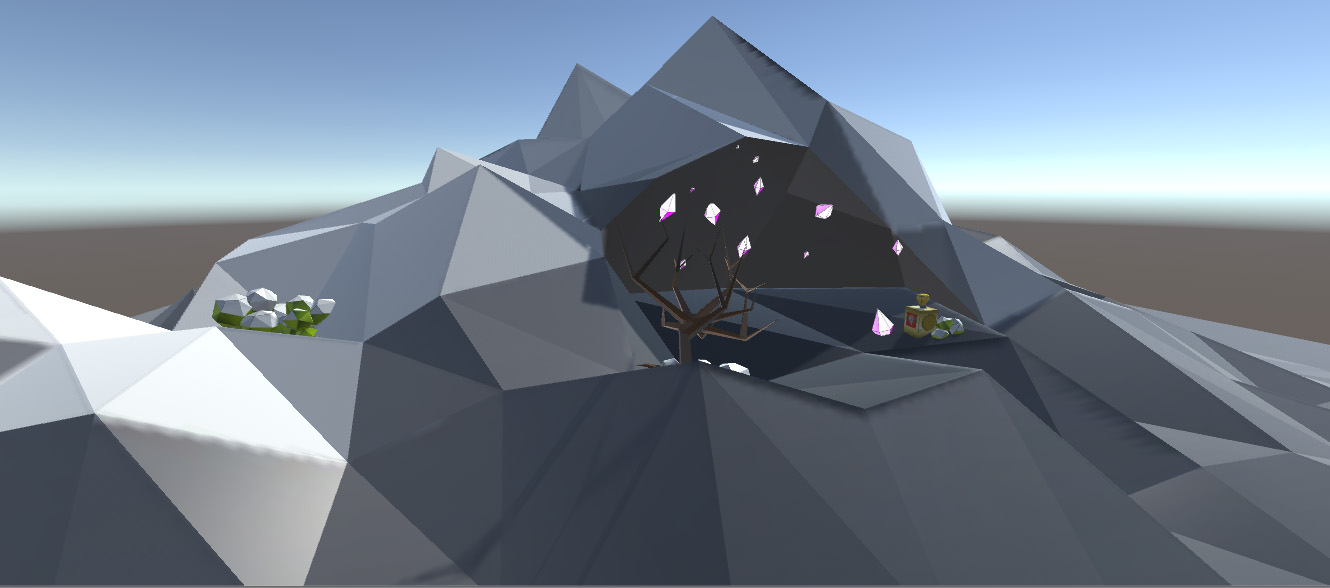
\includegraphics[width=1.0\textwidth]{images/Gebirge}
	\caption{Screenshot der Gebirgslandschaft}
	\label{fig:Gebirge}
\end{figure}

\mysubsubsection{Sandra Beuck}{Dorfwelt}

\begin{figure}[ht]%[htbp]
	\centering
		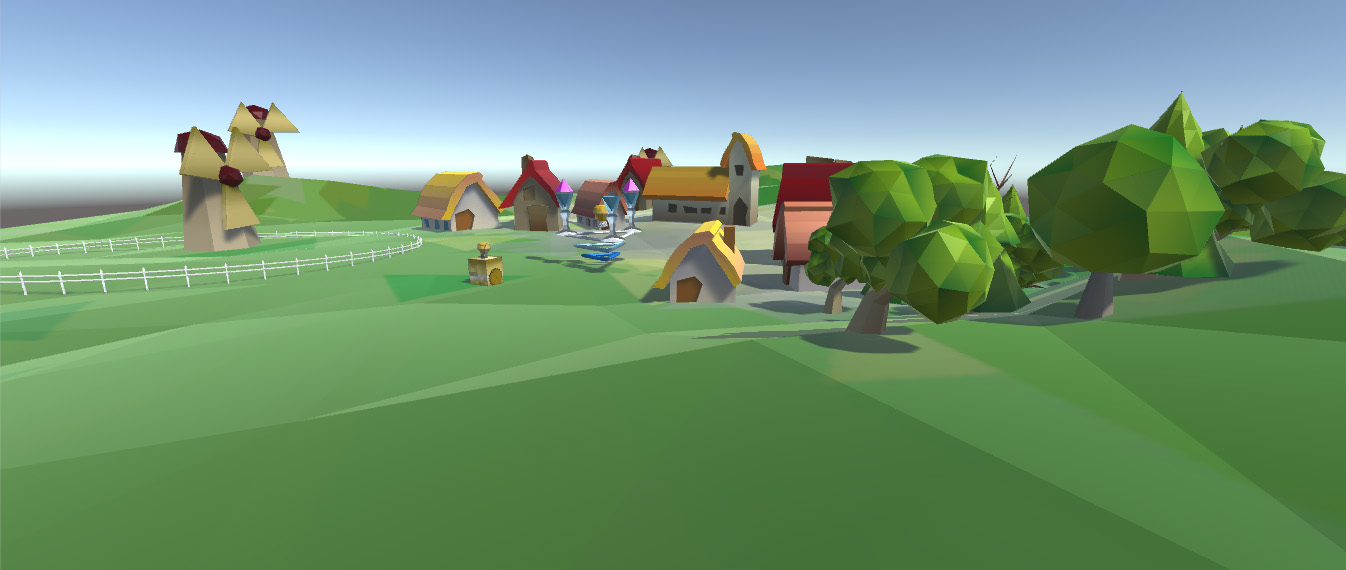
\includegraphics[width=1.0\textwidth]{images/Dorf}
	\caption{Screenshot der Dorflandschaft}
	\label{fig:Dorf}
\end{figure}

\mysubsubsection{Sandra Beuck}{Waldwelt}

\begin{figure}[ht]%[htbp]
	\centering
		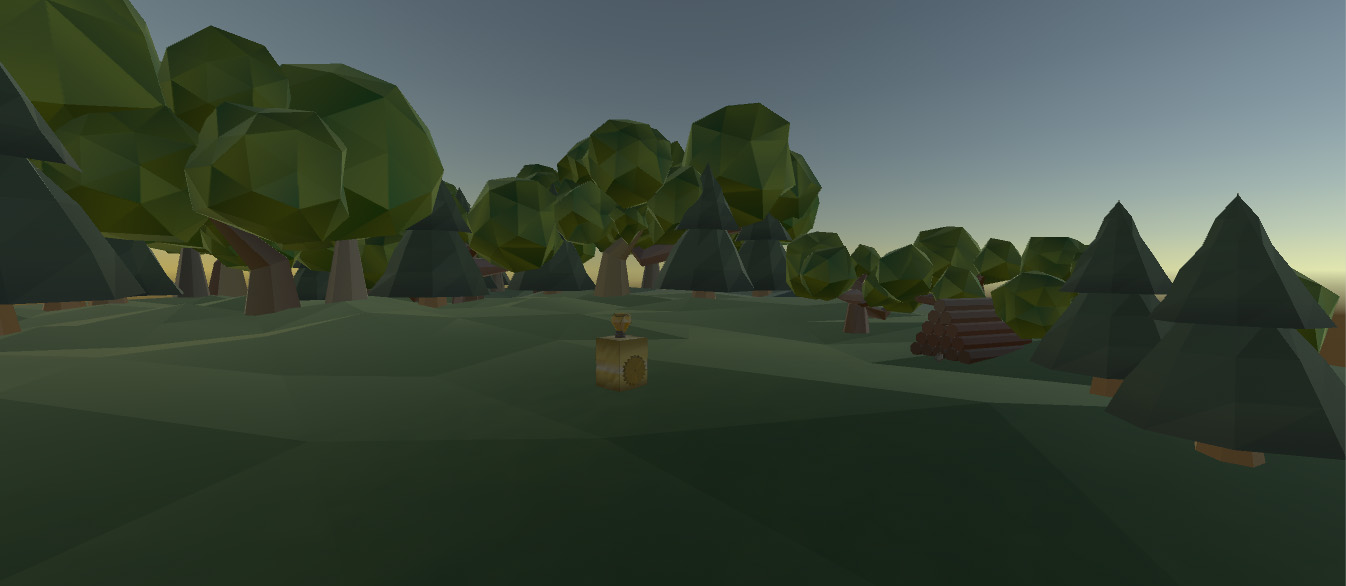
\includegraphics[width=1.0\textwidth]{images/Wald}
	\caption{Screenshot der Waldlandschaft}
	\label{fig:Wald}
\end{figure}

\mysubsubsection{Lydia Friedrich}{Wüstenwelt}

\begin{figure}[ht]%[htbp]
	\centering
		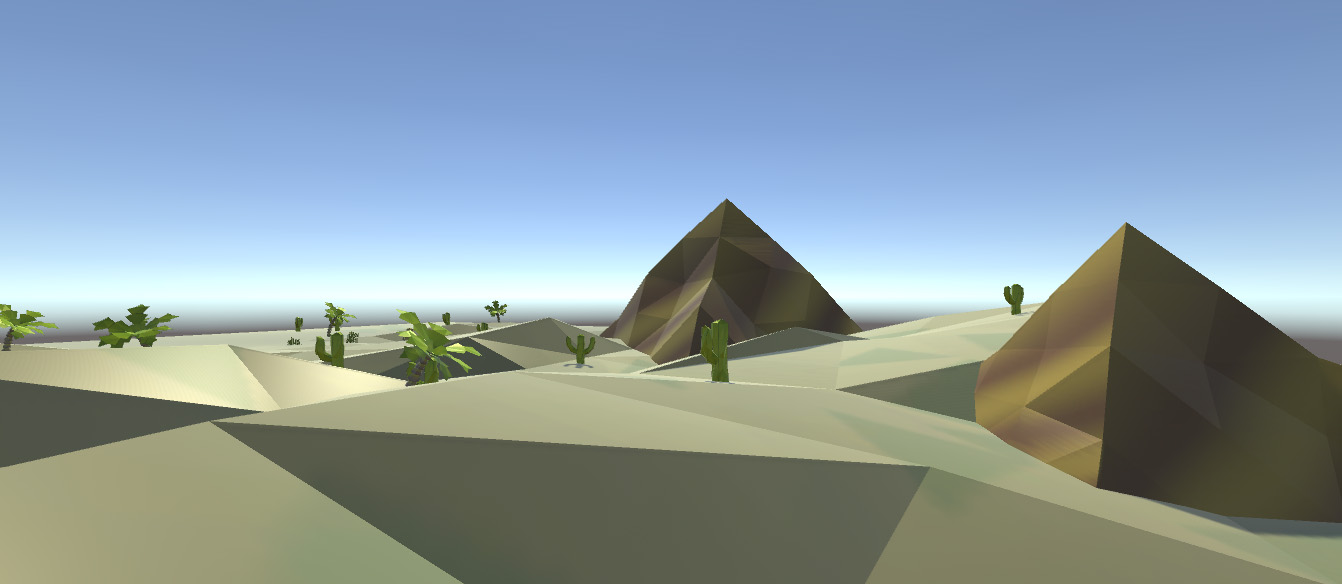
\includegraphics[width=1.0\textwidth]{images/Wueste}
	\caption{Screenshot der Wüstenlandschaft}
	\label{fig:Wueste}
\end{figure}

\mysubsubsection{Sandra Beuck}{Feuerwelt}

\begin{figure}[ht]%[htbp]
	\centering
		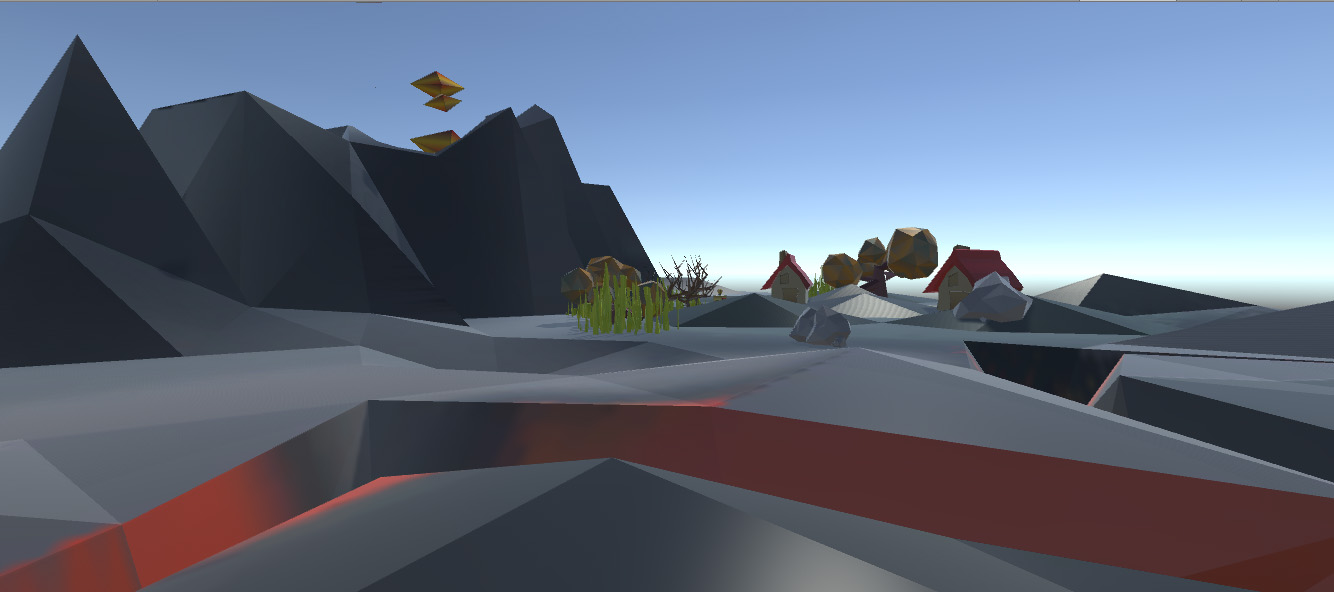
\includegraphics[width=1.0\textwidth]{images/Feuer}
	\caption{Screenshot der Feuerlandschaft}
	\label{fig:Feuer}
\end{figure}

\mysubsubsection{Lydia Friedrich}{Eiswelt}

\begin{figure}[ht]%[htbp]
	\centering
		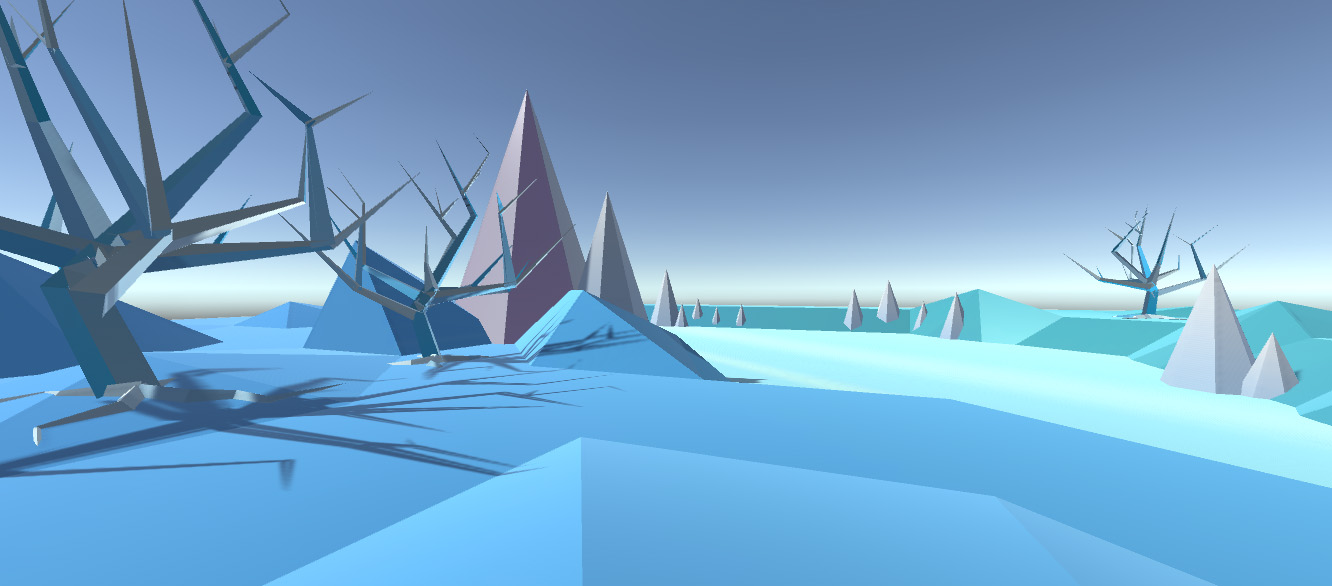
\includegraphics[width=1.0\textwidth]{images/Eis}
	\caption{Screenshot der Eislandschaft}
	\label{fig:Eis}
\end{figure}

\mysubsubsection{Lydia Friedrich}{Skybox}

%\begin{figure}[ht]%[htbp]
%	\centering
%		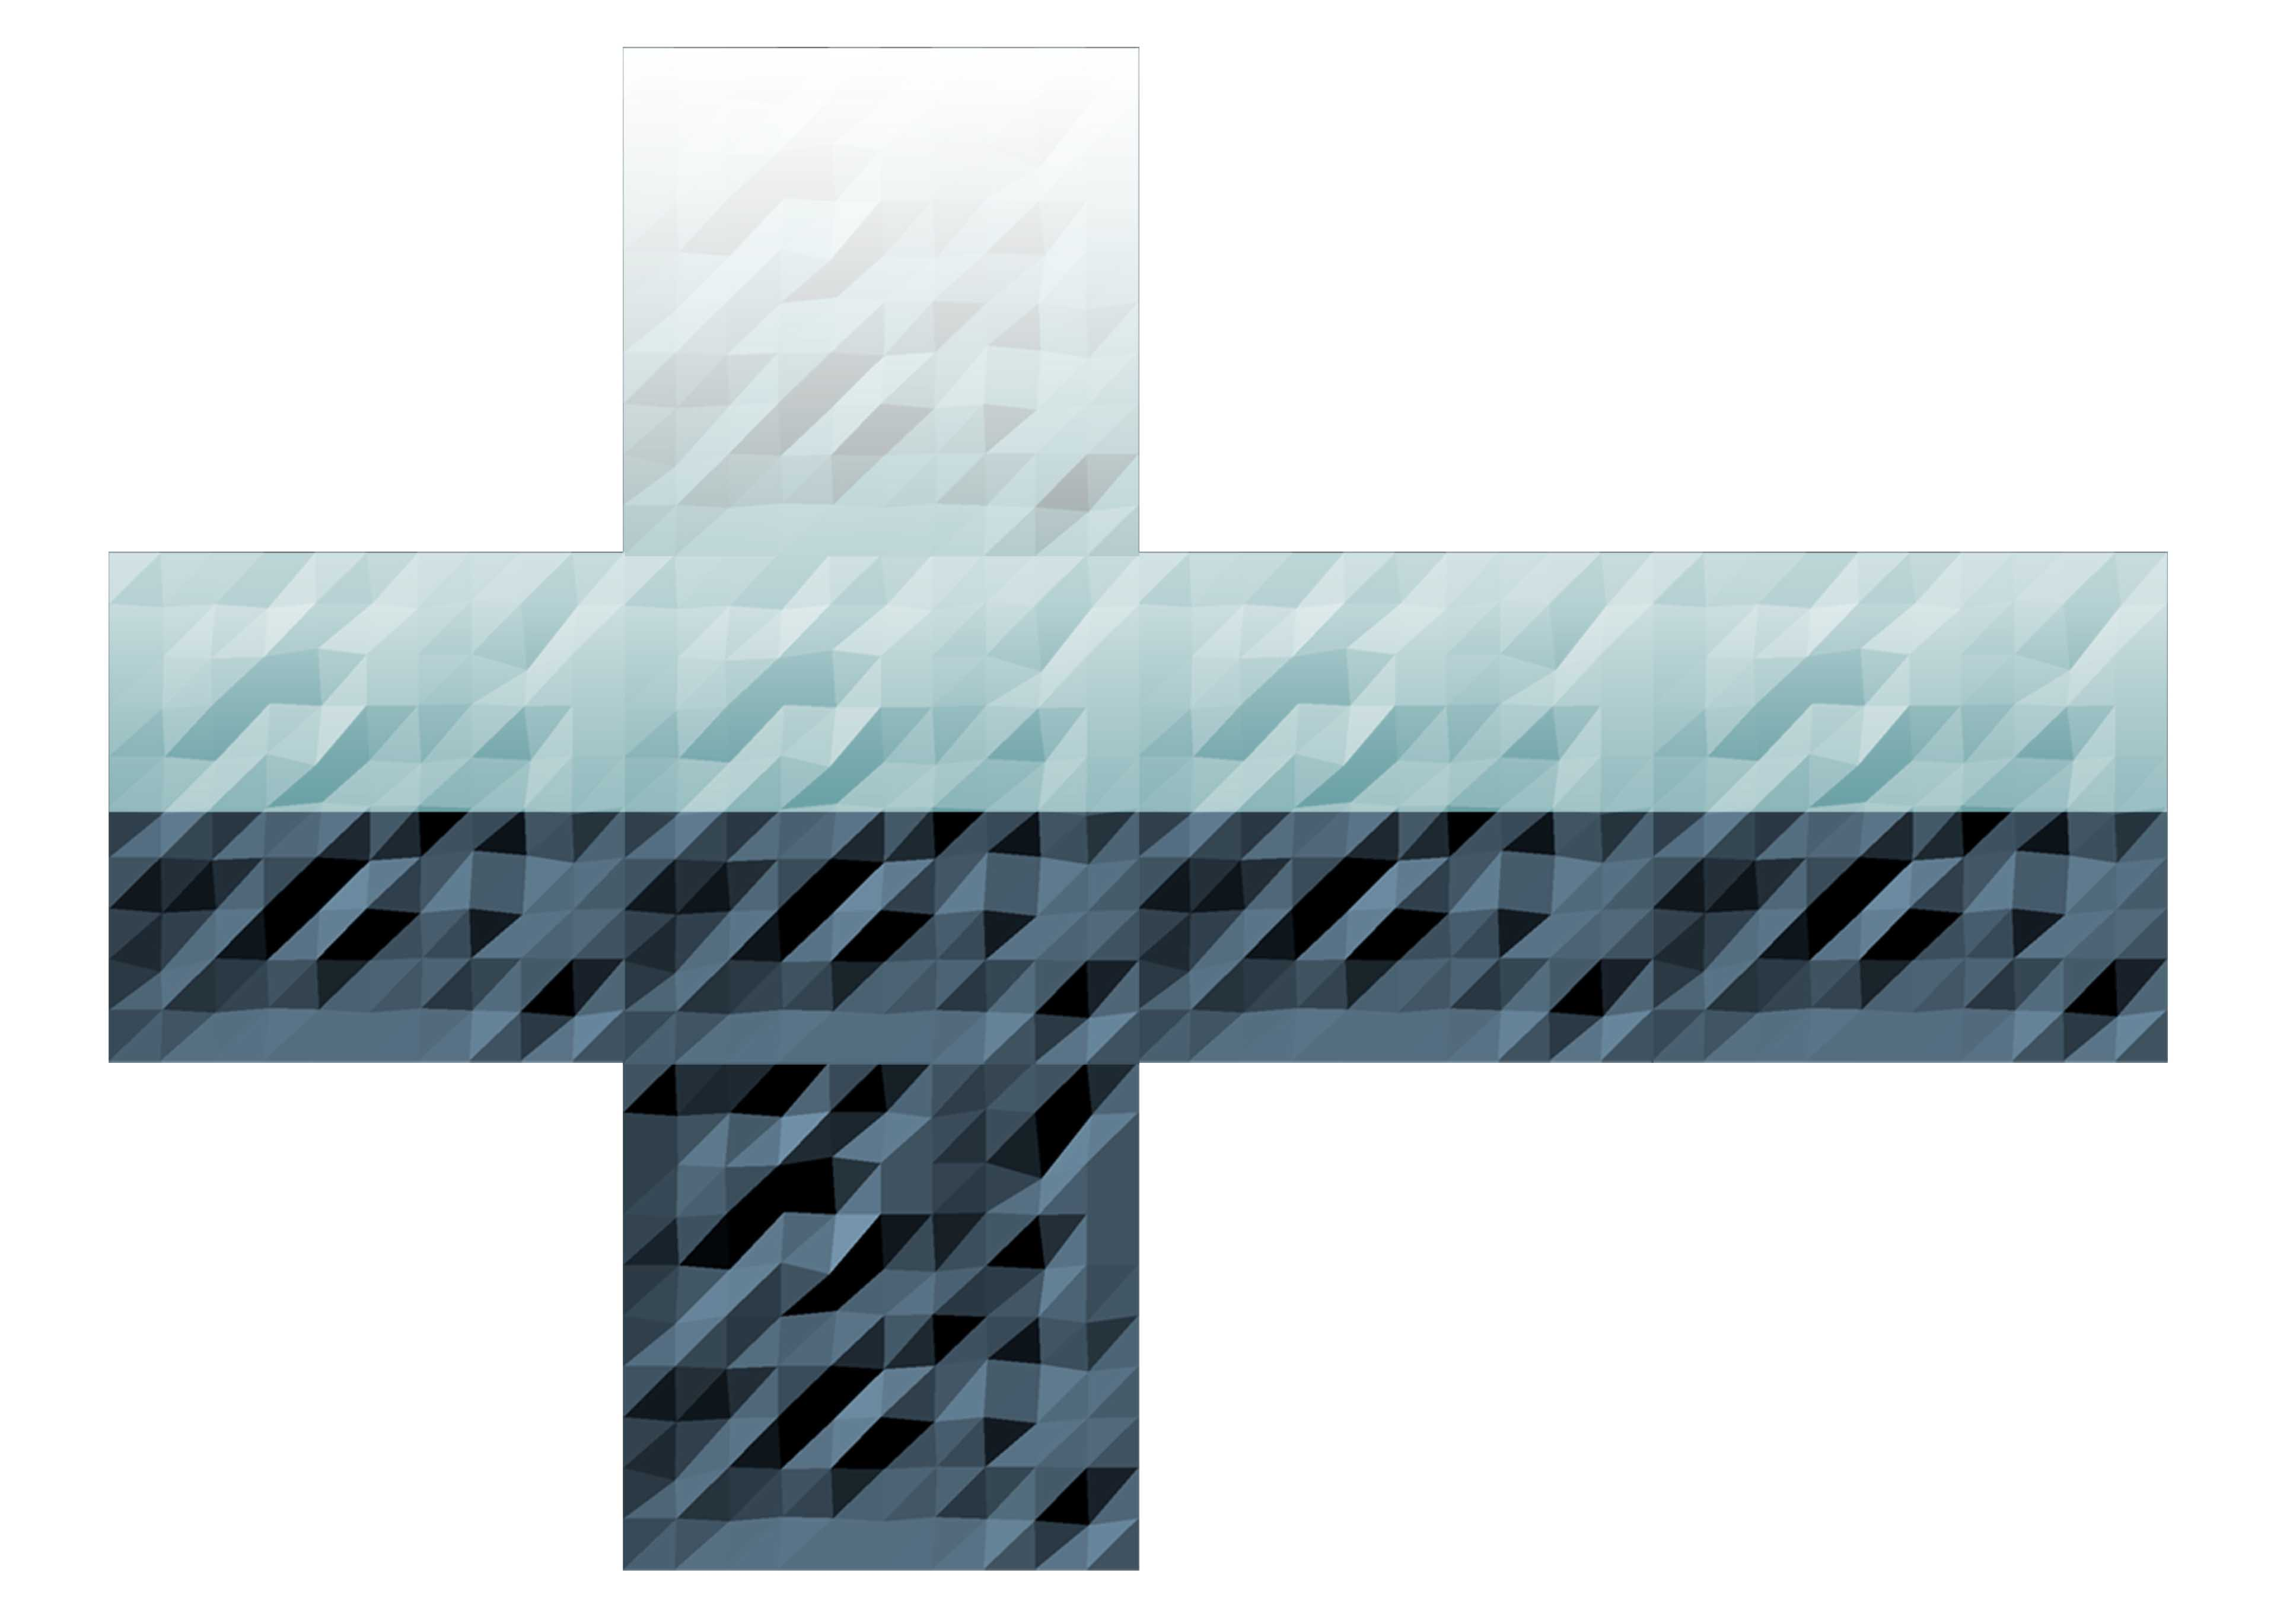
\includegraphics[width=1.0\textwidth]{images/Skybox}
%	\caption{Textur der Skybox}
%	\label{fig:Skybox}
%\end{figure}

SCREENSHOT SKYBOX

Die Skybox (siehe Abbildung \ref{fig:Skybox}) soll den charakteristischen Low Poly Stil des Spiels wiederspiegeln. Um diesen erfolgreich umzusetzen muss ein Würfel in Cinema4D mit Hilfe des Modelling Tools bearbeitet und im Anschluß dessen Textur gebacken werden. Die Textur, welche in einer aufgeklappten Würfelform ausgegeben wird, kann dann in Photoshop nach coleriert werden.